\chapter{Subsystem Services}
\begin{figure}[H]
	\centering
	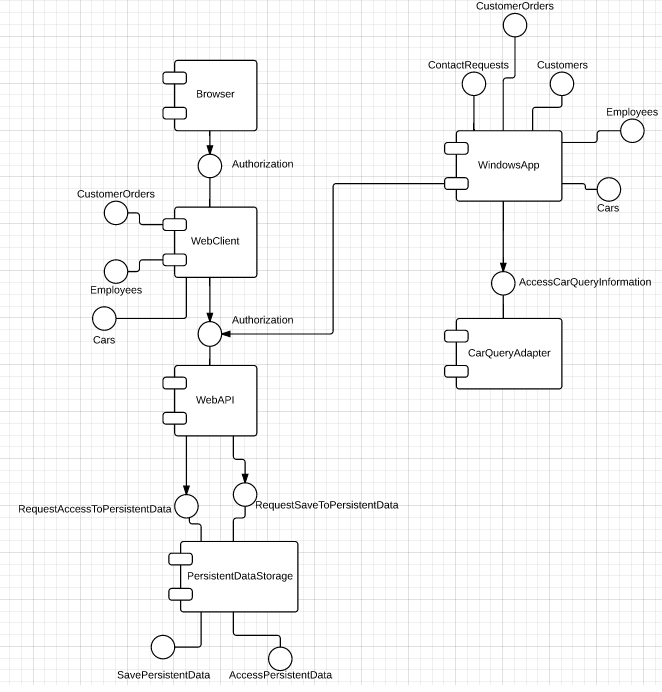
\includegraphics[width=\textwidth]{Figures/SubsystemServices}
	\caption{Services provided by the \texttt{DriveIT} subsystems}
	\label{fig:subsystemservices}
\end{figure}

The above figure shows how the different services of the \texttt{DriveIT System} interact with each other.

The five main subsystems provide ways to contact each other. The main communication happens through the authorisation hooks of the systems, which is illustrated on the figure above.
Data access is also provided by the different services, so that entities can be transferred between services.
